\documentclass{article}
\usepackage[utf8]{inputenc}

\title{Critical Computer Science Reading List}
\author{\textbf{Audrey Beard} \\
        beardj2@rpi.edu \\
        Computer Science Department \\
        Rensselaer Polytechnic Institute}
\date{\today}

\usepackage{natbib}
\usepackage{graphicx}

\newcommand{\etal}{\textit{et al.}}

% Block Quotes \quote{your_text_here}
\usepackage{etoolbox}
\AtBeginEnvironment{quote}{\singlespacing\small}

\begin{document}

\maketitle

\begin{abstract}
    The intent of this document is to provide context for Critical Computer Science Pedagogy at Rensselaer Polytechnic Institute.
    Being rooted in computer vision and machine learning, I undoubtedly bias my literature review towards those topics.
    This document is broken into several sections, ranging from "pure" pedagogical theory, to science and technology studies (STS) literature, to "pure" computer science papers.
\end{abstract}
    
\section{Critiques of CS and Related}
    % 'Good' Isn't Good Enough
    Ben Green's paper \textit{``Good'' Isn't Good Enough}\cite{greenGoodIsnGood2019} is an incisive critique of data science practice, and represents his views that data scientists must think and act critically when performing and thinking about data science.
    He insists that we cannot simply rely on ``good'' or ``ethical'' to guide their work. ``Social good'' in particular is a slippery topic that does not have rigorous definitions and so is often used flexibly to suit business needs.
    This is part of a larger working manifesto of sorts called \textit{Data Science as Political Action}\cite{greenDataSciencePolitical2019}.
    This paper won the Best Paper award in the Public Policy Track at the 2019 NeurIPS Joint Workshop on AI for Social Good.
    
    % Do Artifacts have Politics?
    Langdon Winner's seminal essay \textit{Do Algorithms Have Politics?}\cite{winnerArtifactsHavePolitics1980} explores the claim implied by the title. He posits that artifacts have politics in two distinct ways: as being designed explicitly for some purpose, which reflects the politics of the inventor (the atom bomb, corsets, the Internet, etc.), and as being implicitly reliant \textit{or} implicitly encouraging of specific politics (nuclear power and authoritarianism, solar power and democracy, etc.). It's one of the most-cited STS papers in this space (ethical CS, critical CS, etc.), and is definitely worth reading.

\section{Critical Computer Science Research}
    
    % Designing a moral compass
    Skirpan and Yeh's 2017 paper \textit{Designing a Moral Compass for the Future of Computer Vision Using Speculative Analysis }\cite{skirpanDesigningMoralCompass2017} is concerned with grounding ethics for computer vision in an analysis of potential consequences of a given technology. Their use of \texit{speculative analysis}, a method for exploring a scenario that has not yet occurred via realistic fiction, is particularly notable.
    This tactic is rarely seen in traditional computer vision research, though it is at home in the CVPR Workshops, having appeared in \textit{The Bright and Dark Sides of Computer Vision: Challenges and Opportunities for Privacy and Security}.
    
    % Roles for computing in social change
    \textit{Roles for Computing in Social Change}, by Abebe \etal, identifies four distinct roles computational approaches can fill with respect to affecting social change \cite{abebeRolesComputingSocial2019}. Being an entry in the recent ``tech for good'' movement, this work challenges practitioners in this space to think critically about what is embodied by using a computational solution for a given problem. Without conducting a rigorous inquiry into the possible space of computational approaches to social change, we can draw two meta-conclusions from this work: a) critical computational approaches for social change may be interpreted as filling at least one of these roles, and b) ``social good'' is not accomplished with one-size-fits-all solutions.
    
\section{Computer Science Pedagogy}
    
    % Implementing a Tenth Strand
    \subsection{Implementing a Tenth Strand}
        \textit{Implementing a Tenth Strand in the CS Curriculum} by Martin \etal \cite{martinImplementingTenthStrand1996} offers motivation and suggestions for integrating ethics into computer science curriculum.
        Having been clearly influenced by Schneiderman's keynote address to the ACM SIGCAS Conference \cite{shneidermanHumanValuesFuture1990},
        the case they make is prescriptive of specific ethical values. Though they do not cite feminists or critical race theorists, they do recommend deep integration of ethics with computer science, and call to focus some points that are often ignored in CS classrooms:
        \begin{quote}
        Five basic elements of social analysis are: 1) the social context influences the development and use of technology, 2) power relations are central in all social interaction, 3) technology embodies the values of the developers, 4) populations are always diverse, and 5) empirical data is crucial to the design and development processes.
        \end{quote}
        The authors' sentiment towards modularity is somewhat confusing - they advocate for deep integration of ethical and technical discussion with ``ethics modules''.
        This paper is most useful when viewed as a general overview of how we might integrate discussion, rather than a specific roadmap - it is designed to serve as a set of guidelines for all CS curricula writers.
        
    \subsection{Integrating Ethics within ML Courses}
        \textit{Integrating Ethics within Machine Learning}, by Saltz \etal \cite{saltzIntegratingEthicsMachine2019}, is a recent paper which obviously focuses on machine learning curricula. They specifically highlight the lack of ``ethics'' (the term most commonly used in this space) discussions within classes related to machine learning (including data science and AI). They support this with a systematic literature review (SLR) \cite{kitchenhamGuidelinesPerformingSystematic2007} of syllabi from from the top 20 programs in CS (as ranked by their graduate program by \textit{US News and World Report}).
        
    
%\begin{figure}[h!]
%\centering
%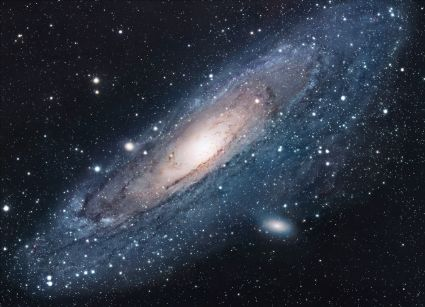
\includegraphics[scale=1.7]{universe}
%\caption{The Universe}
%\label{fig:universe}
%\end{figure}
%
%\section{Conclusion}
%``I always thought something was fundamentally wrong with the universe'' \citep{adams1995hitchhiker}
%
\bibliographystyle{plain}
\bibliography{refs}
\end{document}
